\documentclass[t,serif]{beamer}
\usepackage[portuguese,brazil]{babel} % nomes em portugues
\usepackage[utf8]{inputenc} % acentuacao
\usepackage[T1]{fontenc}
\usepackage{ae} % separacao de sílabas de palavras com acento
\usepackage{icomma}         % acerta espacamento quando a vi­rgula
\usepackage{color}
\usepackage{enumerate}
\usepackage{courier}

\usetheme{Boadilla}
% \usetheme{Copenhagen}
%\usetheme{default}
%\usecolortheme{beaver}
\usecolortheme{seahorse}
\usepackage{textpos}

%%% 1) General Comands
\newcommand{\abf}{\mathbf{a}}
\newcommand{\corr}{\color{red}}
\newcommand{\corb}{\color{blue}}
\newcommand{\corg}{\color{green}}
\newcommand{\cork}{\color{black}}
\newcommand{\cory}{\color{gray}}
\newcommand{\TitleSlide}[1]{\begin{frame} \centering #1 \end{frame}}

% Important constants
\newcommand{\oobf}{\boldsymbol{\o}}
\newcommand{\pibf}{\boldsymbol{\pi}}
\newcommand{\varpibf}{\boldsymbol{\varpi}}

%%% 6) Some operators
\newcommand{\EV}{{\rm E}}          % Expected Value
\newcommand{\TR}{{\rm tr}}         % Trace

\newcommand{\sen}{\textrm{sen}}
\renewcommand{\cos}{\textrm{cos}}
\newcommand{\e}{\textrm{e}}
\newcommand{\cotg}{\textrm{cotg}}
\newcommand{\cosec}{\textrm{cosec}}

\title[StackStorm: Uma Revisão]{\textbf{\underline{StackStorm: Uma Revisão}}}
\subtitle{{\small Tópicos Especiais em Sistemas de Energia Elétrica II: StackStorm\\Prof. Angelo Colombini}}
\author[Rene Cruz Freire]{Rene Cruz Freire}
\date{renefreire@id.uff.br}
\institute[]{Universidade Federal Fluminense\\Campus Niterói}

\setbeamertemplate{blocks}[rounded][shadow=true]
%\setbeamertemplate{footline}[frame number]  %Apaga a linha inferior com o nome do professor
%\setbeamertemplate{page number in head/foot}[totalframenumber]

\begin{document}

% Capa
\frame{
	\vspace*{-0.2cm}
\includegraphics[height=3cm]{figs/escola_eng.png}\hspace*{3.5cm}
\includegraphics[height=3cm]{figs/ppgeet.jpeg}
	\titlepage
}

\addtobeamertemplate{frametitle}{}{%
	\begin{textblock*}{100mm}(.78\textwidth,-1cm)
		\hspace{1.0cm}
\includegraphics[height=1cm]{figs/logo_uff.png}
	\end{textblock*}
}

% Sumário
\section*{Sumário}
	\begin{frame}{Sumário}
		\scriptsize
		\tableofcontents%[pausesections]
	\end{frame}

\section{Introdução}
	\begin{frame}{Introdução}
		\begin{itemize}
			\item Criado em 2014 como uma resposta aos desafios emergentes na automação de operações de TI, especialmente no contexto de DevOps e resposta a eventos em tempo real, o StackStorm é:
		\end{itemize}
		\begin{block}{Documentação oficial do StackStorm}
			``...uma plataforma para integração e automação entre serviços e ferramentas. Ele une sua infraestrutura existente e ambiente de aplicativo para que automatizar esse ambiente mais facilmente. Possui um foco particular em tomar ações em resposta a eventos''
		\end{block}
		\begin{itemize}
			\item O StackStorm é uma plataforma orientada a eventos, sendo regido pela filosofia IFTTT.
			\begin{itemize}
				\item \textbf{IF} \textbf{T}his event happens \textbf{T}hen do \textbf{T}hat.
				\item Se determinado evento ocorre, então faça (uma ação).
			\end{itemize}
		\end{itemize}
	\end{frame}
	
	\begin{frame}{Introdução}
		\begin{itemize}
			\item O StackStorm ajuda a automatizar padrões operacionais comuns, tais como:
			\begin{itemize}
				\item \textit{Deploy} contínuo: se uma nova aplicação for detectada, então faça o \textit{deploy} desta aplicação.
				\item Correção automática: se o servidor parou de responder, então reinicie o servidor.
				\item Notificações: se o tamanho do banco de dados mysql exceder seu limite, então envie uma notificação no e-mail.
			\end{itemize}
			\item O StackStorm auxilia na composição desses e de outros padrões operacionais como regras e fluxos de trabalho (\textit{workflows}), que resultam em ações.
			\item Essas regras e \textit{workflows} são armazenados como código, ou seja, possuem suporte aos sistemas de versionamento hoje utilizados para desenvolvimento, podendo inclusive serem compartilhados com a comunidade \textit{Open Source}.
		\end{itemize}
	\end{frame}

\section{Funcionamento}
	\begin{frame}{Funcionamento}
		\begin{itemize}
			\item O StackStorm se conecta ao ambiente por meio de um conjunto extensível de adaptadores contendo sensores e ações.
		\end{itemize}
		\vspace{0.5cm}
		\begin{center}
			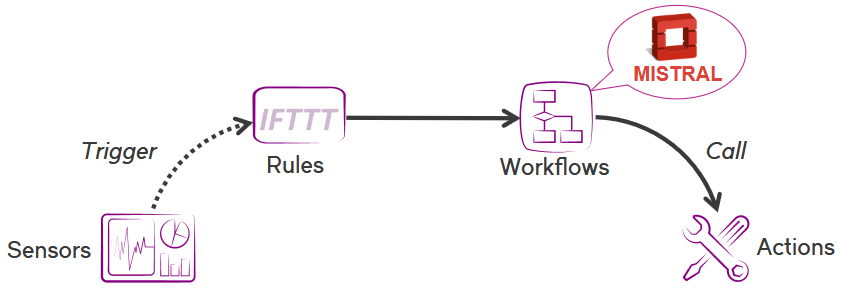
\includegraphics[width=\linewidth]{figs/trab01/1_1.png}
			{\small Fonte: Brocade}
		\end{center}
	\end{frame}
	
	\begin{frame}{Funcionamento}
		\begin{itemize}
			\item Os \textbf{sensores} são plugins Python para integração de entrada ou saída que recebem ou observam eventos, respectivamente. 
			\begin{itemize}
				\item Quando um evento oriundo de sistemas externos ocorre e é processado por um sensor, um \textit{trigger} será emitido para o sistema.
			\end{itemize}
			\item Os \textbf{triggers} são as representações dos eventos externos no ambiente do StackStorm.
			\begin{itemize}
				\item Existem triggers genéricos (por exemplo, timers, webhooks) e triggers de integração (por exemplo, atualização de problemas do JIRA).
				\item Um novo tipo de trigger pode ser definido escrevendo um plugin de sensor.
			\end{itemize}
			\item As \textbf{regras} mapeiam triggers para ações (ou workflows) aplicando critérios de correspondência e mapeando a carga útil do trigger para entradas de ação.
		\end{itemize}
	\end{frame}
	
	\begin{frame}{Funcionamento}
		\begin{itemize}
			\item Um \textbf{Workflow} é um conjunto de ações que define a ordem, condições de transição e passagem dos dados.
			\begin{itemize}
				\item A maioria das automações tem mais de uma etapa e, portanto, precisa de mais de uma ação.
			\end{itemize}
			\item \textbf{Ações} são as integrações de saída do StackStorm, podendo ser plugins Python ou qualquer scripts executado no StackStorm pela inclusão de linhas de metadados.
			\begin{itemize}
				\item As ações podem ser genéricas (ssh, chamada REST), integrações (OpenStack, Docker, Puppet) ou ações personalizadas.
			\end{itemize}
			\item Os \textbf{packs} são as unidades de implantação de conteúdo que estendem o StackStorm.
			 \begin{itemize}
			 	\item Eles simplificam o gerenciamento e o compartilhamento de conteúdo plugável do StackStorm agrupando integrações (triggers e ações) e automações (regras e workflows).
			 \end{itemize}
		\end{itemize}
	\end{frame}
	
	\begin{frame}{Funcionamento}
		\begin{itemize}
			\item Diagrama da arquitetura do StackStorm.
		\end{itemize}
		\begin{center}
			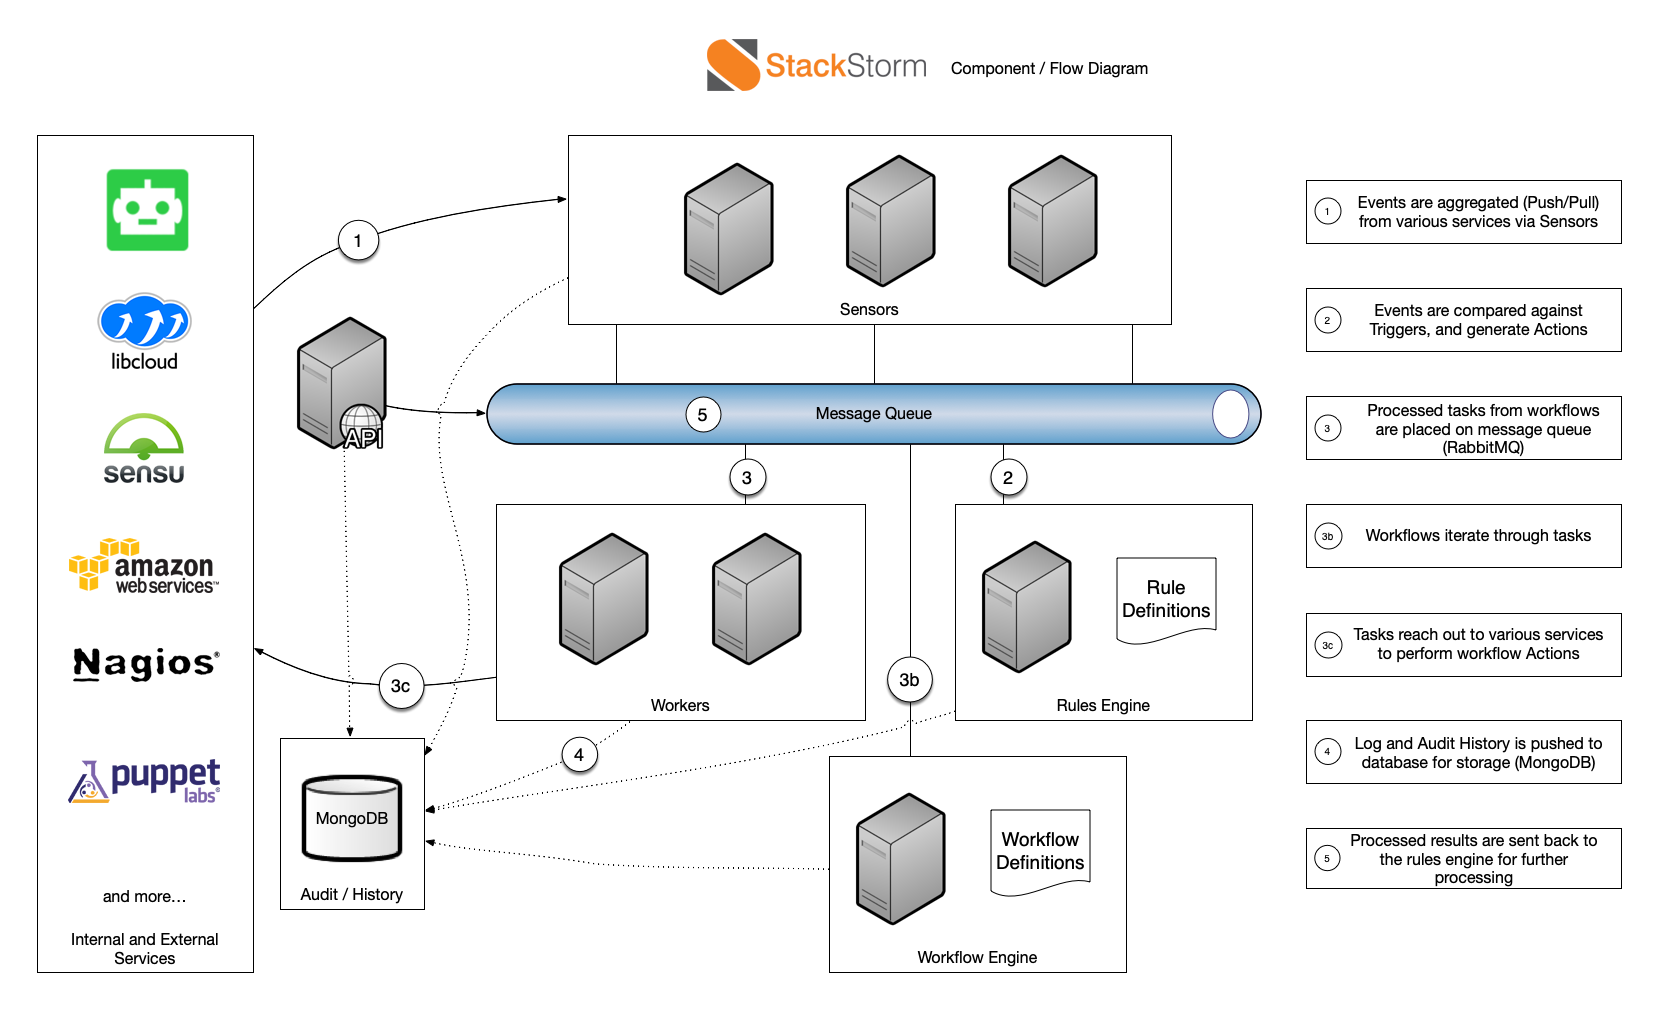
\includegraphics[width=\linewidth]{figs/trab01/1_2.png}
		\end{center}
	\end{frame}
\end{document}
